In this section, will be present
the case where the coronary 
artery has atherosclerosis and 
the drug-eluting stent is placed. 
It is modeled by 10 uniformly spaced 
semi-circles. 
The geometry used promotes a smooth reduction of the 
distance between the upper wall and symmetry axis of the channel. 
Due to atherosclerosis, 40\% channel obstruction was considered 
and the domain was discretized using 15875 nodes and 35408 
linear triangular elements. 

\medskip 
The \ref{velocity evolution curved stent} shows the unsteady state 
velocity profile in the middle section channel, that is, 
$x=5.0R$. 
As expected, the numerical solution tends to a similar profile to
the Half Poiseuille, as presented in the section \ref{half poiseuille sec}. However, it is possible to observe an inversion of the velocity
field sense at the top of the figure.
This inversion occurs in the region that is
located between the stents strut semi-circles.
It is also possible to observe that the maximum horizontal velocity field 
in curvel channel reaches the $u=3.43$ non-dimensional value, that is, 
more than 3 times the blood velocity in coronary artery
without atherosclerosis and stent strut placed. 
This increase can influence the dynamics of blood flow
and its biological processes and a more detailed analysis
should be performed.

\vspace{1cm}
\begin{figure}[H]
     \caption{
The unsteady state velocity profile in the middle ($x=5.0R$) of the curved channel with drug-eluting stent.}
     \centering
     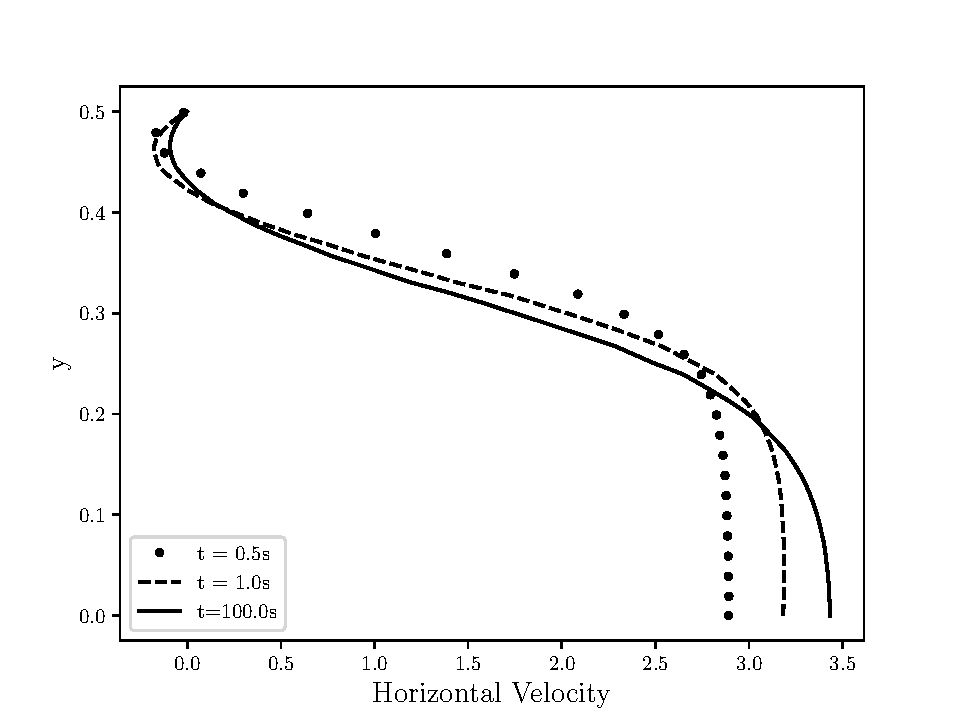
\includegraphics[scale=1]{./02_chaps/cap_solution/figure/vel_CurvedStrut_evol.pdf}\\
     \label{velocity evolution curved stent}
\end{figure}

\newpage
The \ref{velocity field curved stent} presents the evolution in 
time and space of the velocity field for half of the domain
due to the symmetry of the solution. 
The velocity field is represented with non-dimensional values 
where the red color refers to the $u=3.43$ value and the blue color 
$u=0$ value. Conveting to dimensional values, 
we have $u=41.16cm/s$ and $u=0cm/s$ respectively.
As can be seen, the region with the lowest horizontal velocity 
magnitude is found close to the boundary where the no-slip
condition is applied. Whereas, it is increase close to 
the symmetric axis. Moreover, the largest horizontal velocity value
is found in the maximum contraction region.


\vspace{1cm} 
\begin{figure}[H]
     \caption{
Temporal and spatial evolution of the velocity field for curved channel with
drug-eluting stent.}
     \begin{minipage}{.50\linewidth}
      \centering
      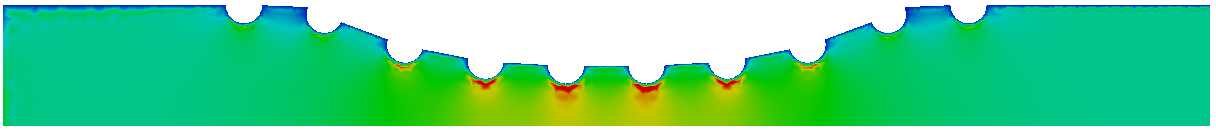
\includegraphics[scale=0.18]{./02_chaps/cap_solution/figure/vel_CurvedStrut1.png}\\
      t = 0.1s
     \end{minipage}%
     \begin{minipage}{.50\linewidth}
      \centering
      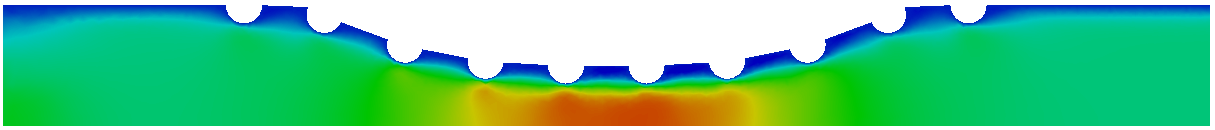
\includegraphics[scale=0.18]{./02_chaps/cap_solution/figure/vel_CurvedStrut2.png}\\
      t = 0.5s
     \end{minipage}
     \begin{minipage}{.50\linewidth}
     \medskip
      \centering
      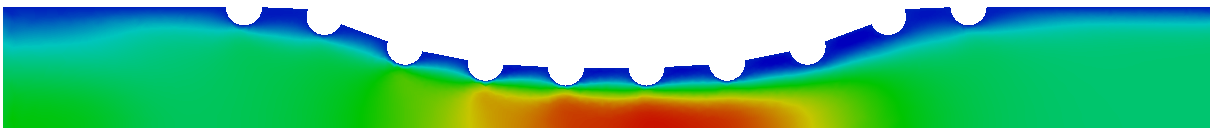
\includegraphics[scale=0.18]{./02_chaps/cap_solution/figure/vel_CurvedStrut3.png}\\
      t = 1.0s
     \end{minipage}%
     \begin{minipage}{.50\linewidth}
     \medskip
      \centering
      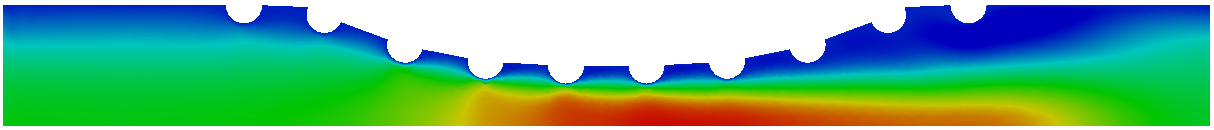
\includegraphics[scale=0.18]{./02_chaps/cap_solution/figure/vel_CurvedStrut4.png}\\
      t = 3.0s
     \end{minipage}
     \begin{minipage}{.50\linewidth}
      \centering
      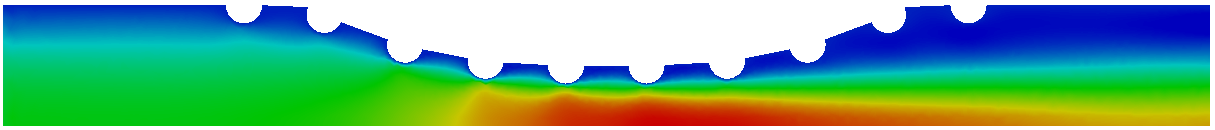
\includegraphics[scale=0.18]{./02_chaps/cap_solution/figure/vel_CurvedStrut5.png}\\
      t = 5.0s
     \end{minipage}%
     \begin{minipage}{.50\linewidth}
      \centering
      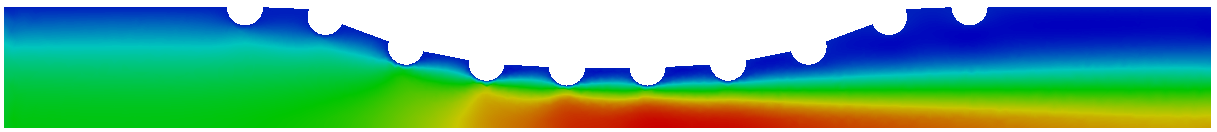
\includegraphics[scale=0.18]{./02_chaps/cap_solution/figure/vel_CurvedStrut6.png}\\
      t = 7.0s
     \end{minipage}
     \begin{minipage}{.50\linewidth}
     \medskip
      \centering
      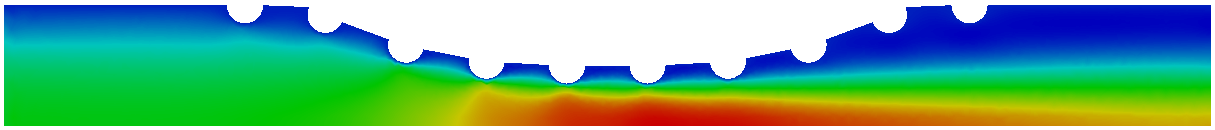
\includegraphics[scale=0.18]{./02_chaps/cap_solution/figure/vel_CurvedStrut7.png}\\
      t = 10.0s
     \end{minipage}%
     \begin{minipage}{.50\linewidth}
     \medskip
      \centering
      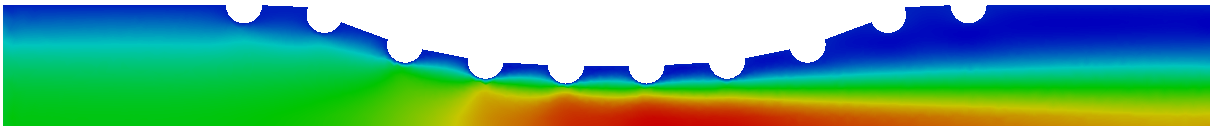
\includegraphics[scale=0.18]{./02_chaps/cap_solution/figure/vel_CurvedStrut8.png}\\
      t = 100.0s
     \end{minipage}\\[10pt]
      \centering
      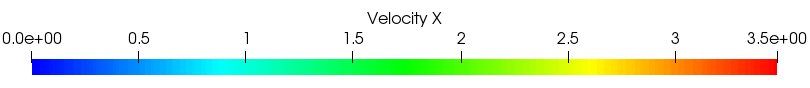
\includegraphics[scale=0.5]{./02_chaps/cap_solution/figure/vel_CurvedStrutScale.png}\\
     \medskip
     \label{velocity field curved stent}
\end{figure}


\vspace{1cm}
As mentioned by Lucena et al. (2018) \cite{lucena2018}, 
it is estimated that 47\% of the drug is diffused to the 
lumem and it is lost to the bloodstream.
The \ref{conc field curved stent sc 1} to 
\ref{conc field curved stent sc 1000} show the temporal and spatial evolution 
of the concentration field for several \textit{Schmidt} number, 
such as: $1$, $10$, $100$ and $1000$ respectively. The concentration field is 
represented with the non-dimensional values where the red color 
represents $100$\% and the blue color represents $0$\% 
of the diffused concentration in the bloodstream. 

\medskip
It is possible to observe in the \ref{conc field curved stent sc 1}
that the concentration field is significally more diffuse than in the
\ref{conc field curved stent sc 10}, where the Schmidt number
is 10 times higher. This means that a large portion of the
diffused drug in bloodstream is quickly spread in the
$Sc=1$ case.
Moreover, in both cases, the concentration field
is more dispersed at the end of the curved channel due to
the sense of the blood flow. It is possible that the
drug concentration diffused affects the density and viscosity of the blood
and consequently the Reynolds number. Thefore, the velocity field would
also be affected. However, this influence is not considered in this work.


\vspace{1cm}
\begin{figure}[H]
     \caption{
Temporal and spatial evolution of the concentration fiel for curved channel with drug-eluting stent and $Sc=1$.}
     \begin{minipage}{.50\linewidth}
      \centering
      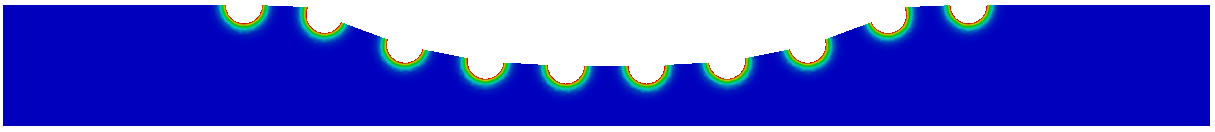
\includegraphics[scale=0.18]{./02_chaps/cap_solution/figure/conc1_CurvedStrut1.png}\\
      t = 0.1s
     \end{minipage}%
     \begin{minipage}{.50\linewidth}
      \centering
      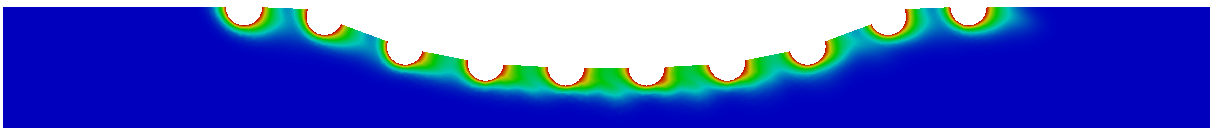
\includegraphics[scale=0.18]{./02_chaps/cap_solution/figure/conc1_CurvedStrut2.png}\\
      t = 0.5s
     \end{minipage}
     \begin{minipage}{.50\linewidth}
     \medskip
      \centering
      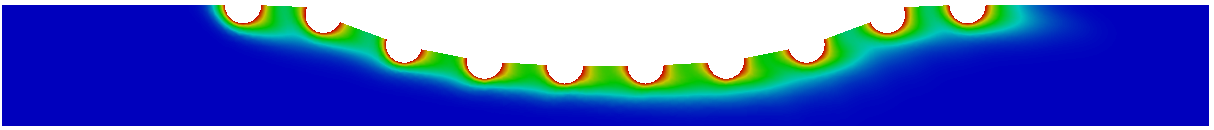
\includegraphics[scale=0.18]{./02_chaps/cap_solution/figure/conc1_CurvedStrut3.png}\\
      t = 1.0s
     \end{minipage}%
     \begin{minipage}{.50\linewidth}
     \medskip
      \centering
      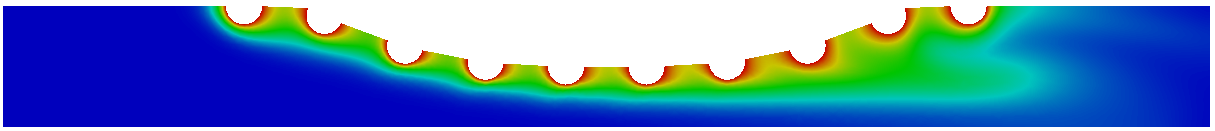
\includegraphics[scale=0.18]{./02_chaps/cap_solution/figure/conc1_CurvedStrut4.png}\\
      t = 3.0s
     \end{minipage}
     \begin{minipage}{.50\linewidth}
      \centering
      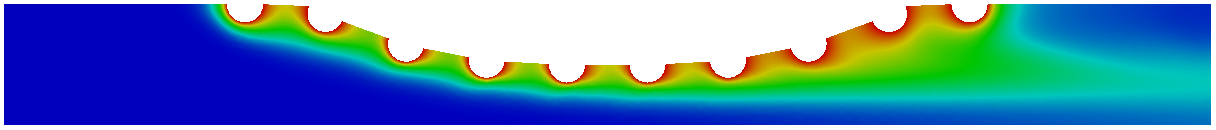
\includegraphics[scale=0.18]{./02_chaps/cap_solution/figure/conc1_CurvedStrut5.png}\\
      t = 5.0s
     \end{minipage}%
     \begin{minipage}{.50\linewidth}
      \centering
      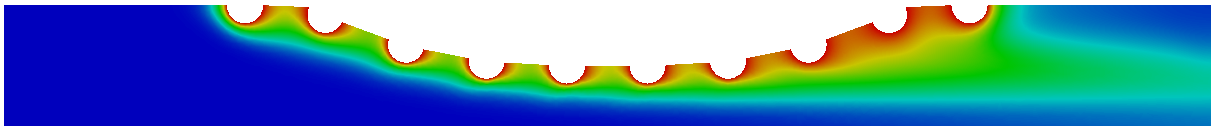
\includegraphics[scale=0.18]{./02_chaps/cap_solution/figure/conc1_CurvedStrut6.png}\\
      t = 7.0s
     \end{minipage}
     \begin{minipage}{.50\linewidth}
     \medskip
      \centering
      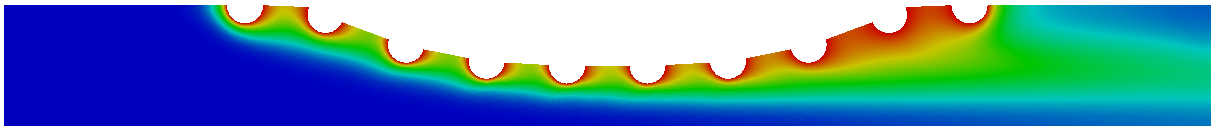
\includegraphics[scale=0.18]{./02_chaps/cap_solution/figure/conc1_CurvedStrut7.png}\\
      t = 10.0s
     \end{minipage}%
     \begin{minipage}{.50\linewidth}
     \medskip
      \centering
      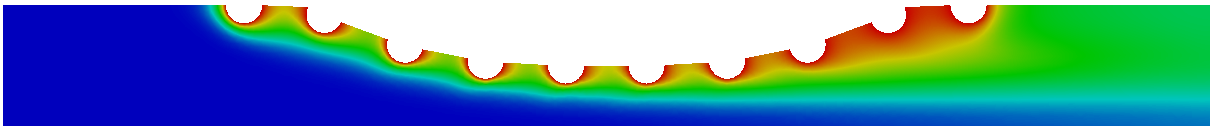
\includegraphics[scale=0.18]{./02_chaps/cap_solution/figure/conc1_CurvedStrut8.png}\\
      t = 100.0s
     \end{minipage}\\[10pt]
      \centering
      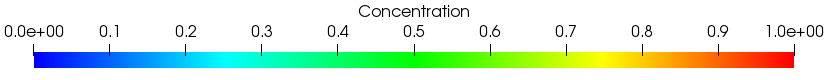
\includegraphics[scale=0.5]{./02_chaps/cap_solution/figure/conc1_CurvedStrutScale.png}\\
     \medskip
     \label{conc field curved stent sc 1}
\end{figure}



\begin{figure}[H]
    \caption{
Temporal and spatial evolution of the concentration fiel for curved channel with drug-eluting stent and $Sc=10$.}
     \begin{minipage}{.50\linewidth}
      \centering
      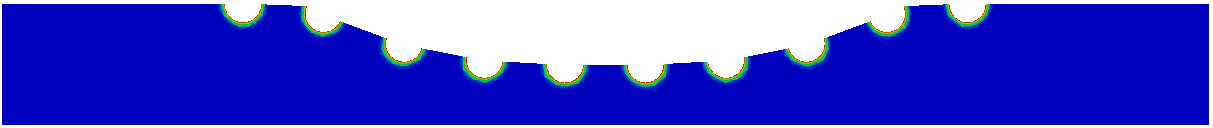
\includegraphics[scale=0.18]{./02_chaps/cap_solution/figure/conc10_CurvedStrut1.png}\\
      t = 0.1s
     \end{minipage}%
     \begin{minipage}{.50\linewidth}
      \centering
      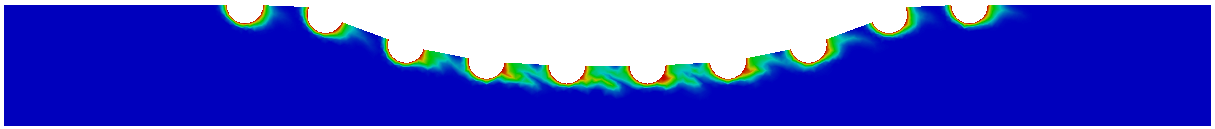
\includegraphics[scale=0.18]{./02_chaps/cap_solution/figure/conc10_CurvedStrut2.png}\\
      t = 0.5s
     \end{minipage}
     \begin{minipage}{.50\linewidth}
     \medskip
      \centering
      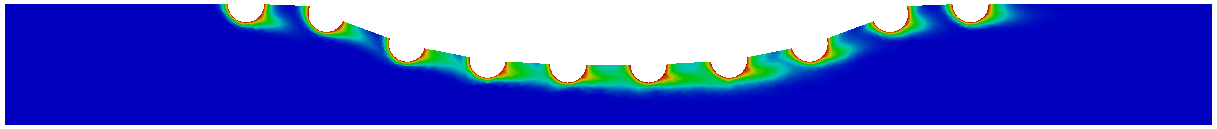
\includegraphics[scale=0.18]{./02_chaps/cap_solution/figure/conc10_CurvedStrut3.png}\\
      t = 1.0s
     \end{minipage}%
     \begin{minipage}{.50\linewidth}
     \medskip
      \centering
      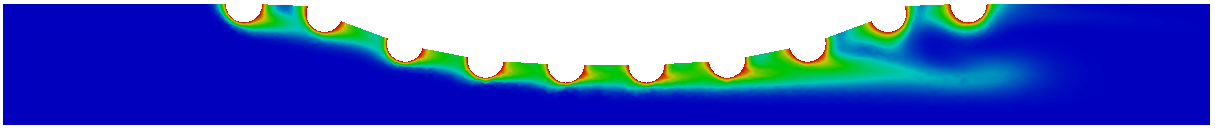
\includegraphics[scale=0.18]{./02_chaps/cap_solution/figure/conc10_CurvedStrut4.png}\\
      t = 3.0s
     \end{minipage}
     \begin{minipage}{.50\linewidth}
      \centering
      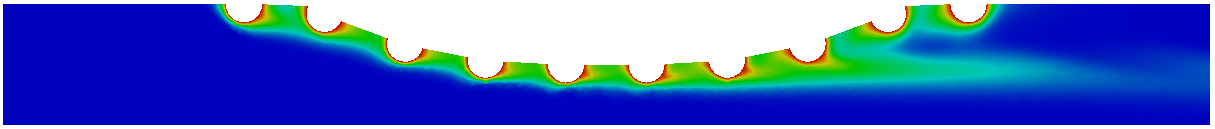
\includegraphics[scale=0.18]{./02_chaps/cap_solution/figure/conc10_CurvedStrut5.png}\\
      t = 5.0s
     \end{minipage}%
     \begin{minipage}{.50\linewidth}
      \centering
      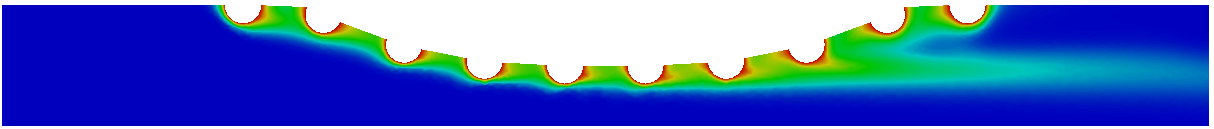
\includegraphics[scale=0.18]{./02_chaps/cap_solution/figure/conc10_CurvedStrut6.png}\\
      t = 7.0s
     \end{minipage}
     \begin{minipage}{.50\linewidth}
     \medskip
      \centering
      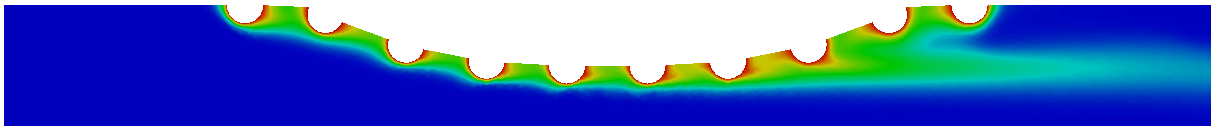
\includegraphics[scale=0.18]{./02_chaps/cap_solution/figure/conc10_CurvedStrut7.png}\\
      t = 10.0s
     \end{minipage}%
     \begin{minipage}{.50\linewidth}
     \medskip
      \centering
      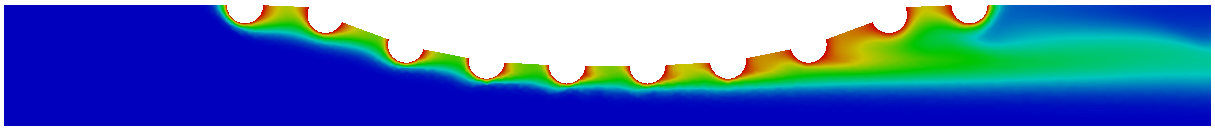
\includegraphics[scale=0.18]{./02_chaps/cap_solution/figure/conc10_CurvedStrut8.png}\\
      t = 100.0s
     \end{minipage}\\[10pt]
      \centering
      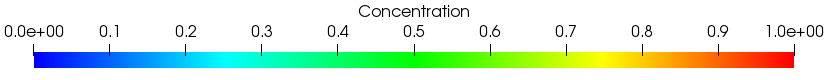
\includegraphics[scale=0.5]{./02_chaps/cap_solution/figure/conc1_CurvedStrutScale.png}\\
     \medskip
     \label{conc field curved stent sc 10}
\end{figure}


\medskip
For the \ref{conc field curved stent sc 100}
and the \ref{conc field curved stent sc 1000},
the Schmidt number is increased to 100 and 1000 respectively.
Both cases have a similar dynamic where it is possible
to observe a decrease in the drug diffusion in the bloodstream
when compared to the previous cases. Another important fact
is the similarity in the concentration field for $Sc=100$
and $Sc=1000$. Therefore, it is necessary to simulate
for longer times. In addition, it is possible to conclude 
that the \textit{Schmidt} number directly 
influences the drug transport in the blood flow and 
for high values of the \textit{Schmidt} number, 
the transport of chemical species becomes purely convective.



\begin{figure}[H]
    \caption{
Temporal and spatial evolution of the concentration fiel for curved channel with drug-eluting stent and $Sc=100$.}
     \begin{minipage}{.50\linewidth}
      \centering
      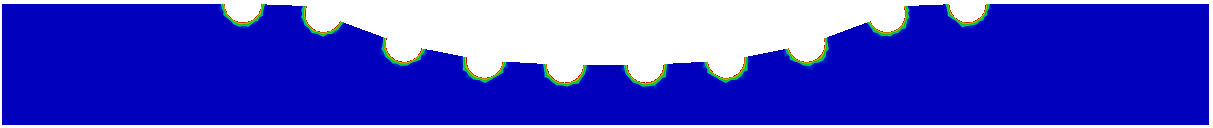
\includegraphics[scale=0.18]{./02_chaps/cap_solution/figure/conc100_CurvedStrut1.png}\\
      t = 0.1s
     \end{minipage}%
     \begin{minipage}{.50\linewidth}
      \centering
      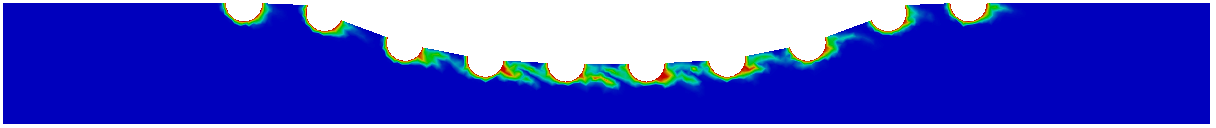
\includegraphics[scale=0.18]{./02_chaps/cap_solution/figure/conc100_CurvedStrut2.png}\\
      t = 0.5s
     \end{minipage}
     \begin{minipage}{.50\linewidth}
     \medskip
      \centering
      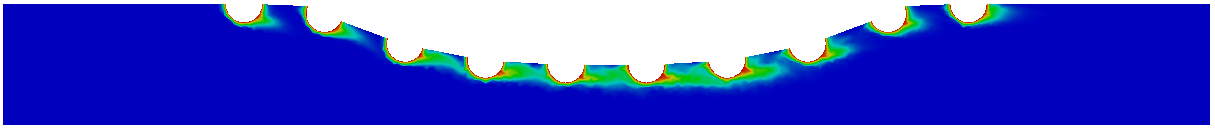
\includegraphics[scale=0.18]{./02_chaps/cap_solution/figure/conc100_CurvedStrut3.png}\\
      t = 1.0s
     \end{minipage}%
     \begin{minipage}{.50\linewidth}
     \medskip
      \centering
      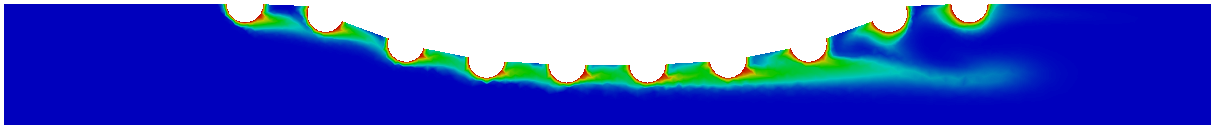
\includegraphics[scale=0.18]{./02_chaps/cap_solution/figure/conc100_CurvedStrut4.png}\\
      t = 3.0s
     \end{minipage}
     \begin{minipage}{.50\linewidth}
      \centering
      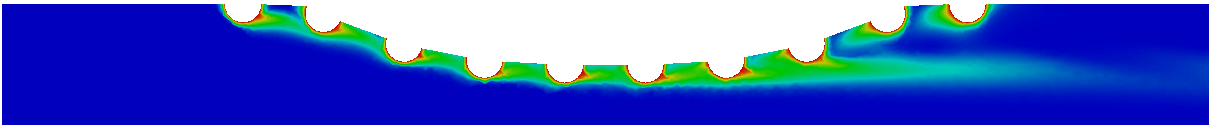
\includegraphics[scale=0.18]{./02_chaps/cap_solution/figure/conc100_CurvedStrut5.png}\\
      t = 5.0s
     \end{minipage}%
     \begin{minipage}{.50\linewidth}
      \centering
      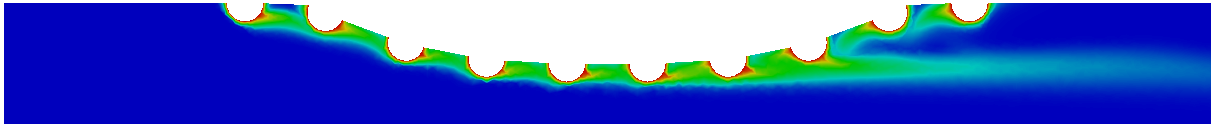
\includegraphics[scale=0.18]{./02_chaps/cap_solution/figure/conc100_CurvedStrut6.png}\\
      t = 7.0s
     \end{minipage}
     \begin{minipage}{.50\linewidth}
     \medskip
      \centering
      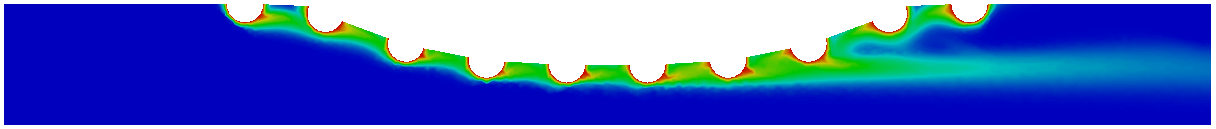
\includegraphics[scale=0.18]{./02_chaps/cap_solution/figure/conc100_CurvedStrut7.png}\\
      t = 10.0s
     \end{minipage}%
     \begin{minipage}{.50\linewidth}
     \medskip
      \centering
      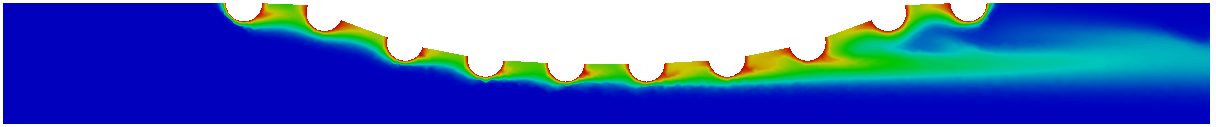
\includegraphics[scale=0.18]{./02_chaps/cap_solution/figure/conc100_CurvedStrut8.png}\\
      t = 100.0s
     \end{minipage}\\[10pt]
      \centering
      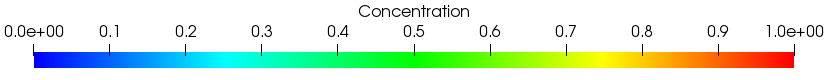
\includegraphics[scale=0.5]{./02_chaps/cap_solution/figure/conc1_CurvedStrutScale.png}\\
     \medskip
     \label{conc field curved stent sc 100}
\end{figure}

\begin{figure}[H]
    \caption{
Temporal and spatial evolution of the concentration fiel for curved channel with drug-eluting stent and $Sc=1000$.}
     \begin{minipage}{.50\linewidth}
      \centering
      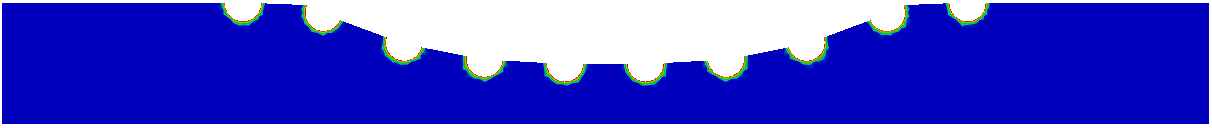
\includegraphics[scale=0.18]{./02_chaps/cap_solution/figure/conc1000_CurvedStrut1.png}\\
      t = 0.1s
     \end{minipage}%
     \begin{minipage}{.50\linewidth}
      \centering
      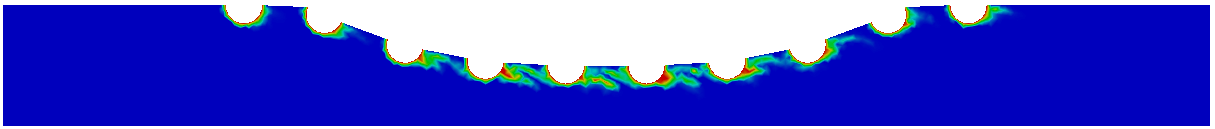
\includegraphics[scale=0.18]{./02_chaps/cap_solution/figure/conc1000_CurvedStrut2.png}\\
      t = 0.5s
     \end{minipage}
     \begin{minipage}{.50\linewidth}
     \medskip
      \centering
      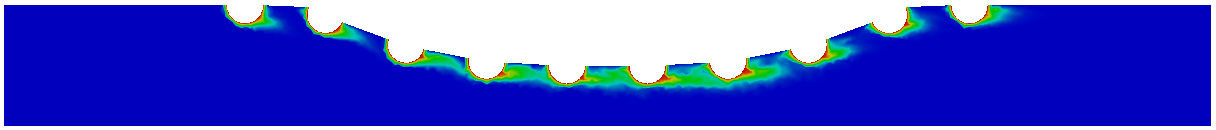
\includegraphics[scale=0.18]{./02_chaps/cap_solution/figure/conc1000_CurvedStrut3.png}\\
      t = 1.0s
     \end{minipage}%
     \begin{minipage}{.50\linewidth}
     \medskip
      \centering
      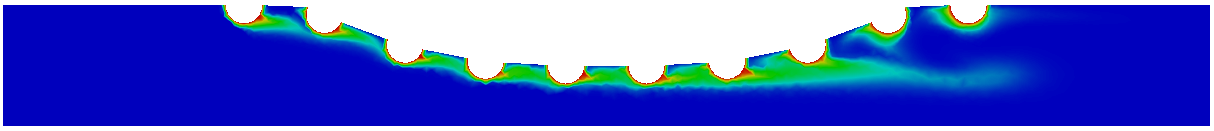
\includegraphics[scale=0.18]{./02_chaps/cap_solution/figure/conc1000_CurvedStrut4.png}\\
      t = 3.0s
     \end{minipage}
     \begin{minipage}{.50\linewidth}
      \centering
      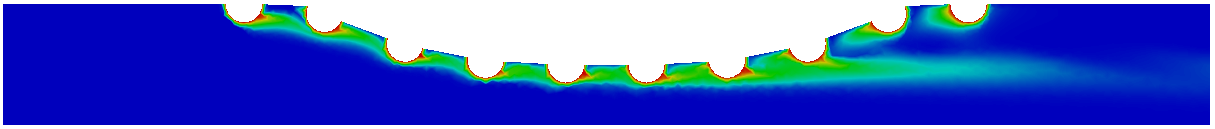
\includegraphics[scale=0.18]{./02_chaps/cap_solution/figure/conc1000_CurvedStrut5.png}\\
      t = 5.0s
     \end{minipage}%
     \begin{minipage}{.50\linewidth}
      \centering
      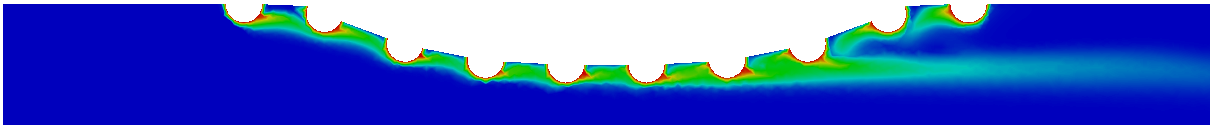
\includegraphics[scale=0.18]{./02_chaps/cap_solution/figure/conc1000_CurvedStrut6.png}\\
      t = 7.0s
     \end{minipage}
     \begin{minipage}{.50\linewidth}
     \medskip
      \centering
      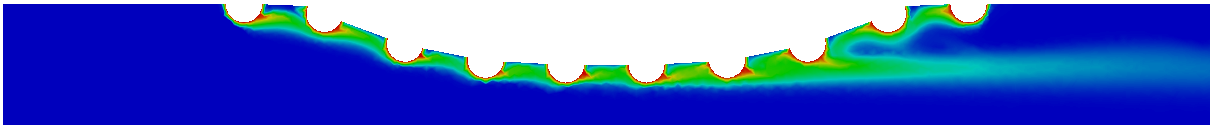
\includegraphics[scale=0.18]{./02_chaps/cap_solution/figure/conc1000_CurvedStrut7.png}\\
      t = 10.0s
     \end{minipage}%
     \begin{minipage}{.50\linewidth}
     \medskip
      \centering
      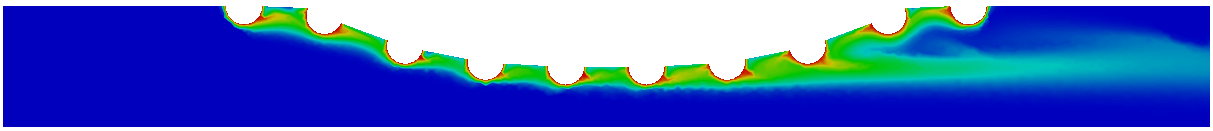
\includegraphics[scale=0.18]{./02_chaps/cap_solution/figure/conc1000_CurvedStrut8.png}\\
      t = 100.0s
     \end{minipage}\\[10pt]
      \centering
      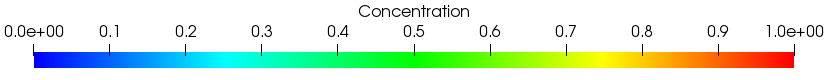
\includegraphics[scale=0.5]{./02_chaps/cap_solution/figure/conc1_CurvedStrutScale.png}\\
     \medskip
     \label{conc field curved stent sc 1000}
\end{figure}



\bigskip
------------------------------------------------------------
Quad

\vspace{1cm}
\begin{figure}[H]
     \caption{
Temporal and spatial evolution of the concentration fiel for curved channel with drug-eluting stent and $Sc=1$.}
     \begin{minipage}{.50\linewidth}
      \centering
      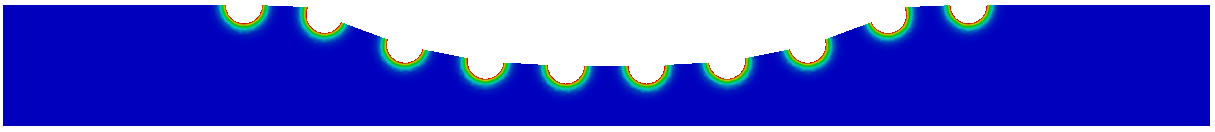
\includegraphics[scale=0.18]{./02_chaps/cap_solution/figure/conc1_CurvedStrut1.png}\\
      t = 0.1s
     \end{minipage}%
     \begin{minipage}{.50\linewidth}
      \centering
      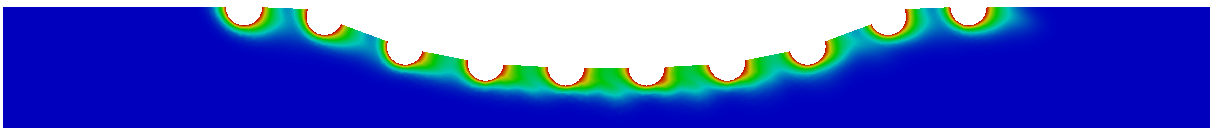
\includegraphics[scale=0.18]{./02_chaps/cap_solution/figure/conc1_CurvedStrut2.png}\\
      t = 0.5s
     \end{minipage}
     \begin{minipage}{.50\linewidth}
     \medskip
      \centering
      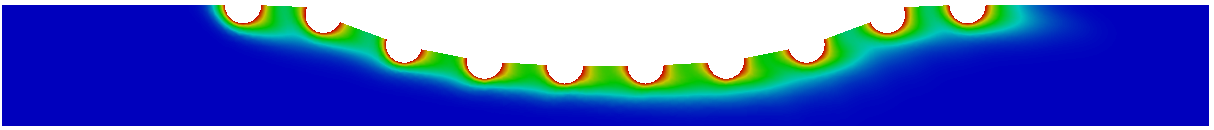
\includegraphics[scale=0.18]{./02_chaps/cap_solution/figure/conc1_CurvedStrut3.png}\\
      t = 1.0s
     \end{minipage}%
     \begin{minipage}{.50\linewidth}
     \medskip
      \centering
      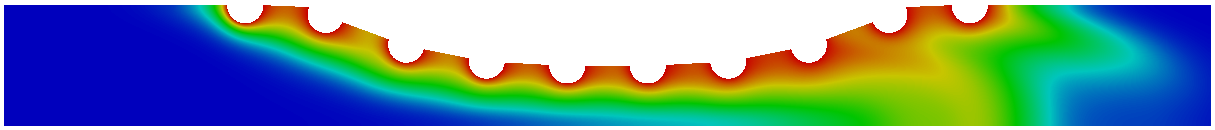
\includegraphics[scale=0.18]{./02_chaps/cap_solution/figure/conc1_quadCurvedStrut4.png}\\
      t = 3.0s
     \end{minipage}
     \begin{minipage}{.50\linewidth}
      \centering
      \includegraphics[scale=0.18]{./02_chaps/cap_solution/figure/conc1_quadCurvedStrut5.png}\\
      t = 5.0s
     \end{minipage}%
     \begin{minipage}{.50\linewidth}
      \centering
      \includegraphics[scale=0.18]{./02_chaps/cap_solution/figure/conc1_quadCurvedStrut6.png}\\
      t = 7.0s
     \end{minipage}
     \begin{minipage}{.50\linewidth}
     \medskip
      \centering
      \includegraphics[scale=0.18]{./02_chaps/cap_solution/figure/conc1_quadCurvedStrut7.png}\\
      t = 10.0s
     \end{minipage}%
     \begin{minipage}{.50\linewidth}
     \medskip
      \centering
      \includegraphics[scale=0.18]{./02_chaps/cap_solution/figure/conc1_quadCurvedStrut8.png}\\
      t = 100.0s
     \end{minipage}\\[10pt]
      \centering
      \includegraphics[scale=0.5]{./02_chaps/cap_solution/figure/conc1_CurvedStrutScale.png}\\
     \medskip
     \label{quad conc field curved stent sc 1}
\end{figure}



